\documentclass[10pt]{beamer}
\usetheme[numbering=fraction,titleformat=smallcaps,progressbar=frametitle]{metropolis}

\usepackage[english]{babel}
\usepackage{graphicx}
\usepackage{wrapfig}
\usepackage{longtable}
\usepackage{ulem}       % underline/strikethrough
\usepackage{tikzsymbols} % smileys
\usepackage{fontawesome5}

\title{Instrument Similarity Analysis\\Stage 1 -- Proposal (CMP223)}
\author{Enrico Dal Pizzol \\ UFRGS / INF / PPGC}
\date{\today}

\begin{document}

\maketitle

\begin{frame}{Computational Object}
\textbf{Object}: Methods for measuring similarity and correlation between financial time series. \\[0.3cm]

\textbf{Goal}: Evaluate computational performance of different algorithms (execution time, CPU, memory). \\[0.3cm]

\textbf{Methods}: Pearson, Spearman, Kendall, DTW (and optionally MI).
\end{frame}

\begin{frame}{Motivation}
\begin{itemize}
  \item Correlation influences risk, diversification, and trading decisions.
  \item Different methods $\Rightarrow$ different assumptions \& costs
  \item Pearson: linear, very fast
  \item Spearman/Kendall: monotonic, robust to outliers
  \item DTW: handles misalignment, but much heavier
\end{itemize}
\end{frame}


\begin{frame}{Computational Object --- Characteristics}
\begin{itemize}
  \item Depending on the chosen period and frequency, time series can become very large.
  \item Each algorithm has its own computational cost and statistical properties.
  \item The task is the comparison of two financial time series.
  \item Each correlation/similarity method has specific strengths:
    \begin{itemize}
      \item Good for capturing linear trends (Pearson)
      \item Robust to outliers and non-linearity (Spearman/Kendall)
      \item Suitable for comparing series that are distorted or shifted in time (DTW)
    \end{itemize}
\end{itemize}
\end{frame}



\begin{frame}{Analysis Method (Measurement)}
\begin{itemize}
  \item Apply correlation methods on real or replayed financial time series
  \item Environment \& tools: Python (NumPy, Pandas, SciPy) and Docker
  \item Metrics collected: correlation output, CPU usage (avg/peak), memory, and execution time
\end{itemize}
\end{frame}


\begin{frame}{Parameters }
\begin{itemize}
  \item Period: 1d, 7d, 1m, 6m, 1y
  \item Frequency: 1s, 1min, 1h, 1d
  \item Method: Pearson, Spearman, Kendall, DTW
  \item Instruments: X, Y, Z (pairs)
  \item Purpose: compare trade-offs: accuracy × computational cost
\end{itemize}
\end{frame}

\begin{frame}{Metrics (What will be measured)}
\begin{itemize}
      \item Execution time
      \item CPU usage (\%)
      \item Avg/Peak memory 
      \item \textbf{Correlation variance}
    \end{itemize}
\end{frame}

\begin{frame}{Experiment Orchestration}
\begin{itemize}
  \item Input: CSV with all parameter combinations
  \item Runner: one container per row
  \item Inside container: calculate correlation
  \item Collector: monitor CPU \& memory
  \item Aggregator: merge into \texttt{results.csv}
\end{itemize}
\end{frame}

\begin{frame}{Experiment Pipeline}
\begin{center}
  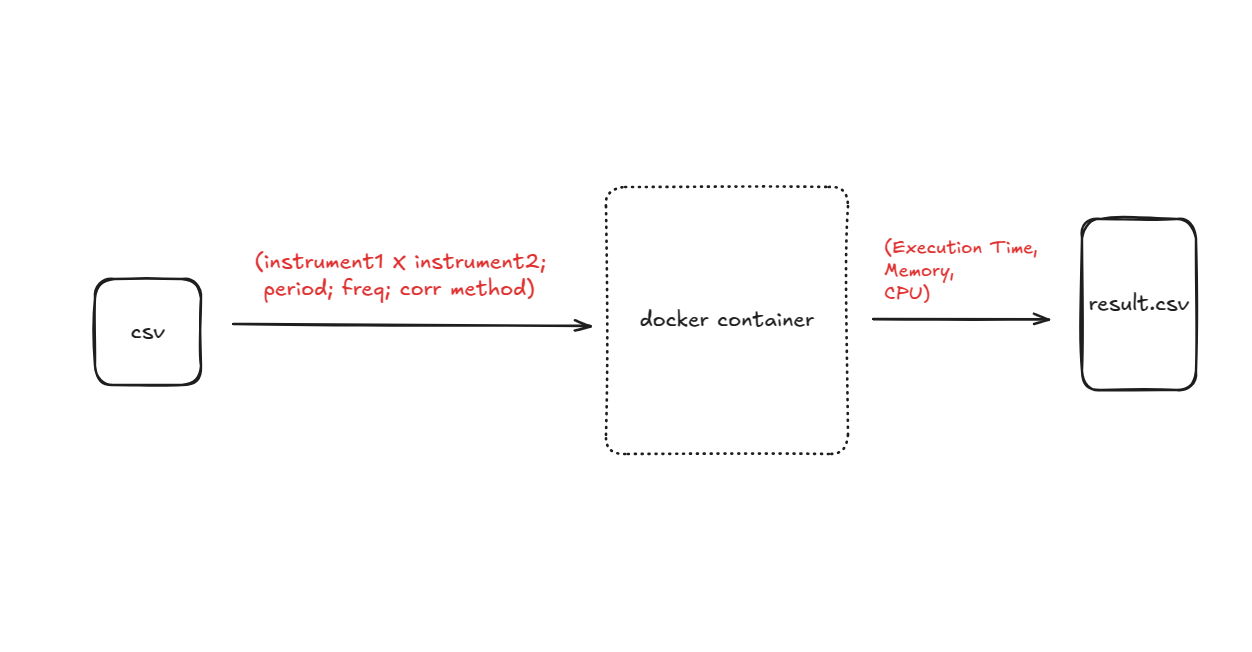
\includegraphics[width=0.9\linewidth]{diagram.png}
\end{center}
\end{frame}


\begin{frame}{Example Result (Mock)}
\begin{tabular}{|l|l|l|l|l|l|l|}
\hline
Instruments & Period & Freq & Method & Time & Mem & CPU \\
\hline
X×Y & 1d & 1min & Pearson & 0.01s & 5MB & 2\% \\
X×Y & 1d & 1min & Spearman & 0.03s & 6MB & 3\% \\
X×Y & 7d & Daily & Kendall & 0.02s & 5MB & 2\% \\
X×Z & 6m & 1s & DTW & 2h & 700MB & 45\% \\
\hline
\end{tabular}
\end{frame}

\begin{frame}{Next-Steps Schedule (8 Weeks)}
\begin{itemize}
  \item W1: Collect dataset and preprocess
  \item W2-3: Build test suite (Docker, scripts, ...)
  \item W4--6: Run experiments; record metrics
  \item W7: Analyze results; generate plots/tables
  \item W8: Write and submit final report
\end{itemize}
\end{frame}

\begin{frame}{Q\&A}
\begin{center}
Thank you! \\[0.5cm]
\faGithub\ \href{https://github.com/enricopizzol/instrument-similarity-analysis}{\texttt{instrument-similarity-analysis}}
\end{center}
\end{frame}


\begin{frame}{References}
\scriptsize
\begin{thebibliography}{9}

\bibitem{bader2021}
Alexander Bader. \textit{How can we quantify similarity between time series?}, Gorilla Tech Blog, May 27, 2021.  
Available at: \url{https://tech.gorilla.co/how-can-we-quantify-similarity-between-time-series-ed1d0b633ca0}

\bibitem{medium2020}
Ishan Jain. \textit{Choosing the Right Correlation: Pearson vs Spearman vs Kendall’s Tau}.  
Available at: \url{https://ishanjainoffical.medium.com/choosing-the-right-correlation-pearson-vs-spearman-vs-kendalls-tau-02dc7d7dd01d}

\bibitem{puspita2020}
P. E. Puspita and Zulkarnain, 
\textit{A Practical Evaluation of Dynamic Time Warping in Financial Time Series Clustering},  
2020 International Conference on Advanced Computer Science and Information Systems (ICACSIS), Depok, Indonesia, 2020, pp. 61–68.  
doi: \href{https://doi.org/10.1109/ICACSIS51025.2020.9263123}{10.1109/ICACSIS51025.2020.9263123}

\bibitem{winistorfer2023}
M. Winistörfer and I. Zhdankin, 
\textit{Measure of Dependence for Financial Time-Series},  
arXiv preprint 2023.  
Available at: \url{https://arxiv.org/abs/2311.12129}

\end{thebibliography}
\end{frame}


\end{document}
